
\subsubsection{5.1 H-E3: Per-Sample Hessian Trace Discriminates Minority Group Membership}

\textbf{Main result:} 4/5 seeds satisfy all three gate criteria simultaneously. The H-E3 existence gate is satisfied.

\#\#\#\# Per-Seed AUROC Results

\begin{table*}[htbp]
\centering
\resizebox{\dimexpr 2\columnwidth+\columnsep\relax}{!}{%
\begin{tabular}{lllllllllll}
\toprule
Seed & AUROC(t=0) & t=1 & t=5 & t=10 & t=20 & t=50 & t* & AUROC(t*) & Spearman $\rho$ & Pass \\
\midrule
1 & 0.538 & 0.838 & 0.657 & 0.780 & 0.850 & 0.879 & 20 & 0.850 & 0.70 & ✗ \\
2 & 0.609 & 0.671 & 0.827 & 0.825 & 0.844 & 0.885 & 50 & 0.885 & 0.943 & ✓ \\
3 & 0.558 & 0.459 & 0.580 & 0.797 & 0.860 & 0.897 & 50 & 0.897 & 0.943 & ✓ \\
4 & 0.579 & 0.568 & 0.799 & 0.853 & 0.903 & 0.905 & 20 & 0.903 & 0.900 & ✓ \\
5 & 0.609 & 0.735 & 0.890 & 0.875 & 0.840 & 0.916 & 5 & 0.890 & 1.000 & ✓ \\
\bottomrule
\end{tabular}
}
\end{table*}

\textbf{Gate result: PASS (4/5 seeds).} Seed 1 fails due to a non-monotone AUROC trajectory (Spearman $\rho$=0.70, threshold 0.80) caused by a dip at t=5 --- both AUROC(t=0)<0.70 and AUROC(t*)$\geq 0.85$ are satisfied for seed 1, but the Spearman criterion is not.

\textbf{Epoch-0 control (RQ2):} All 5 seeds show AUROC(t=0) $\in$ [0.538, 0.609] (mean 0.577) --- well below the 0.70 control threshold. The pretrained ImageNet backbone alone does not discriminate minority from majority training samples on Waterbirds. The trace asymmetry is created by ERM training.

\textbf{Comparison context:} This paper establishes the existence result (AUROC>0.85) for the per-sample Hessian trace signal. A direct AUROC comparison against first-order annotation-free proxies (JTT-proxy, SELF) is left for future work, as such baselines require implementing and running their minority detection pipelines under identical conditions. The epoch-0 AUROC $\in$ [0.538, 0.609] provides a lower bound from the pretrained baseline.

\begin{figure}[htbp]
\centering
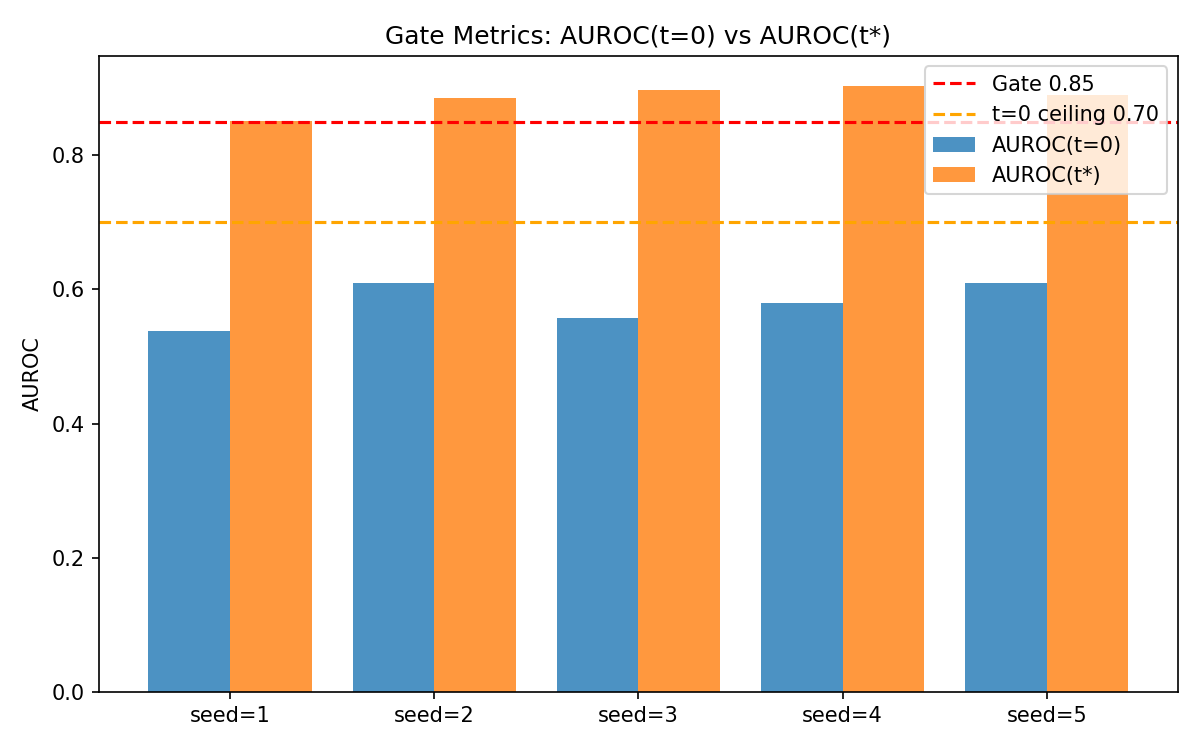
\includegraphics[width=\columnwidth]{figures/fig1_gate_metrics.png}
\caption{AUROC at t* and epoch-0 per seed with gate thresholds}
\label{fig:fig1_gate_metrics}
\end{figure}

\textit{Figure 1: AUROC at t} and epoch-0 per seed with gate thresholds (0.70 and 0.85). All 5 seeds show epoch-0 AUROC below 0.70 (mean 0.577), confirming ERM-induced signal. Four of five seeds achieve AUROC(t\textit{)$\geq 0.85$.}

\#\#\#\# Trace Ratio R(t)

The trace ratio R(t) = mean\_minority\_trace / mean\_majority\_trace rises from near-unity at initialization to peak values of 4.09--8.89:

\begin{table*}[htbp]
\centering
\resizebox{\dimexpr 2\columnwidth+\columnsep\relax}{!}{%
\begin{tabular}{lllllllll}
\toprule
Seed & R(t=0) & R(t=1) & R(t=5) & R(t=10) & R(t=20) & R(t=50) & t* & R(t*) \\
\midrule
1 & 1.05 & 3.78 & 0.88 & 1.36 & 4.37 & 3.74 & 20 & 4.37 \\
2 & 1.12 & 2.31 & 3.36 & 2.85 & 2.06 & 5.55 & 50 & 5.55 \\
3 & 1.06 & 1.23 & 1.10 & 2.55 & 2.93 & 7.21 & 50 & 7.21 \\
4 & 1.08 & 1.41 & 2.99 & 3.20 & 4.09 & 3.13 & 20 & 4.09 \\
5 & 1.12 & 3.02 & 8.89 & 4.12 & 1.10 & 2.60 & 5 & 8.89 \\
\bottomrule
\end{tabular}
}
\end{table*}

All seeds show $R(t)>>1$ --- minority Hessian traces are systematically higher than majority at the peak checkpoint. Optimal $t^*$ varies across seeds ($t^*\in \{5, 20, 50\}$), indicating that the peak of minority-majority curvature divergence is stochastic across training runs. Seeds 2 and 3 show R still increasing at t=50, and no clear decline is observed within the checkpoint schedule --- the peak-then-decline pattern assumed at hypothesis formulation is not universal.

\begin{figure}[htbp]
\centering
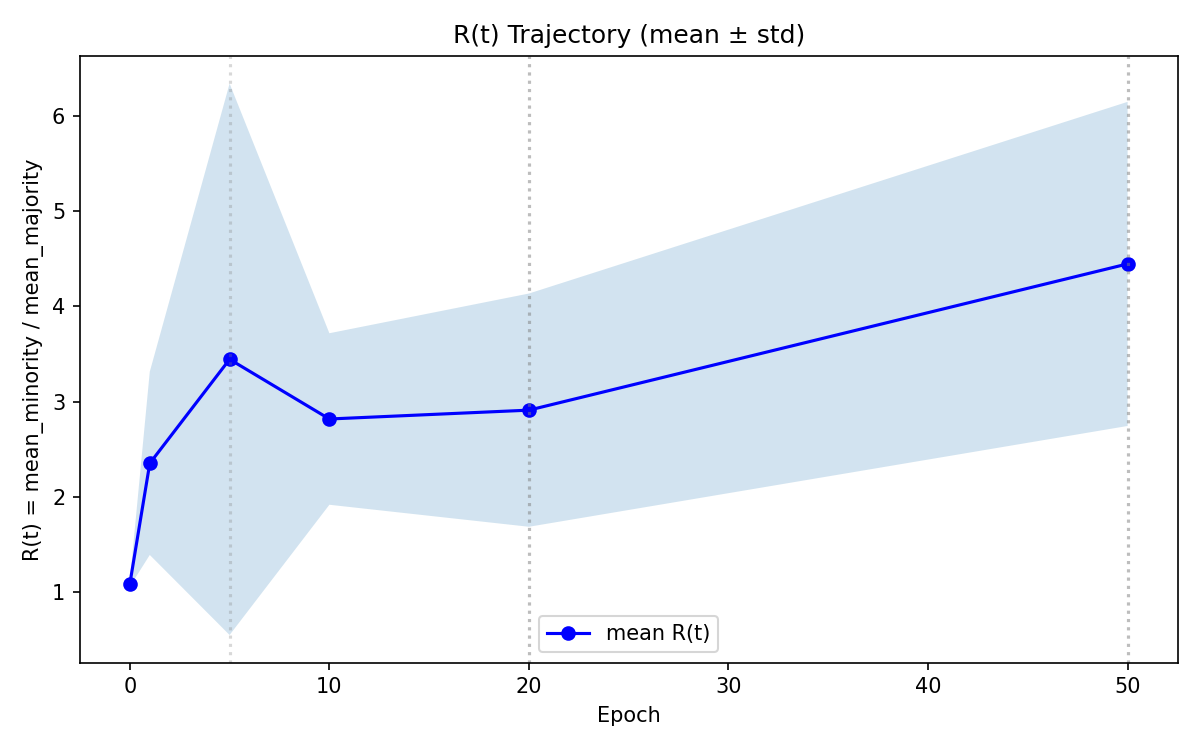
\includegraphics[width=\columnwidth]{figures/fig2_R_trajectory.png}
\caption{R(t) trajectory across training epochs}
\label{fig:fig2_R_trajectory}
\end{figure}

\textit{Figure 2: Trace ratio R(t) = mean\_minority\_trace(t) / mean\_majority\_trace(t) across training epochs for all 5 seeds. R rises from near-unity at initialization ($R\approx 1.05$--1.12) to peak values of 4.09--8.89, with t} varying across {5, 20, 50} depending on seed.*

\begin{figure}[htbp]
\centering
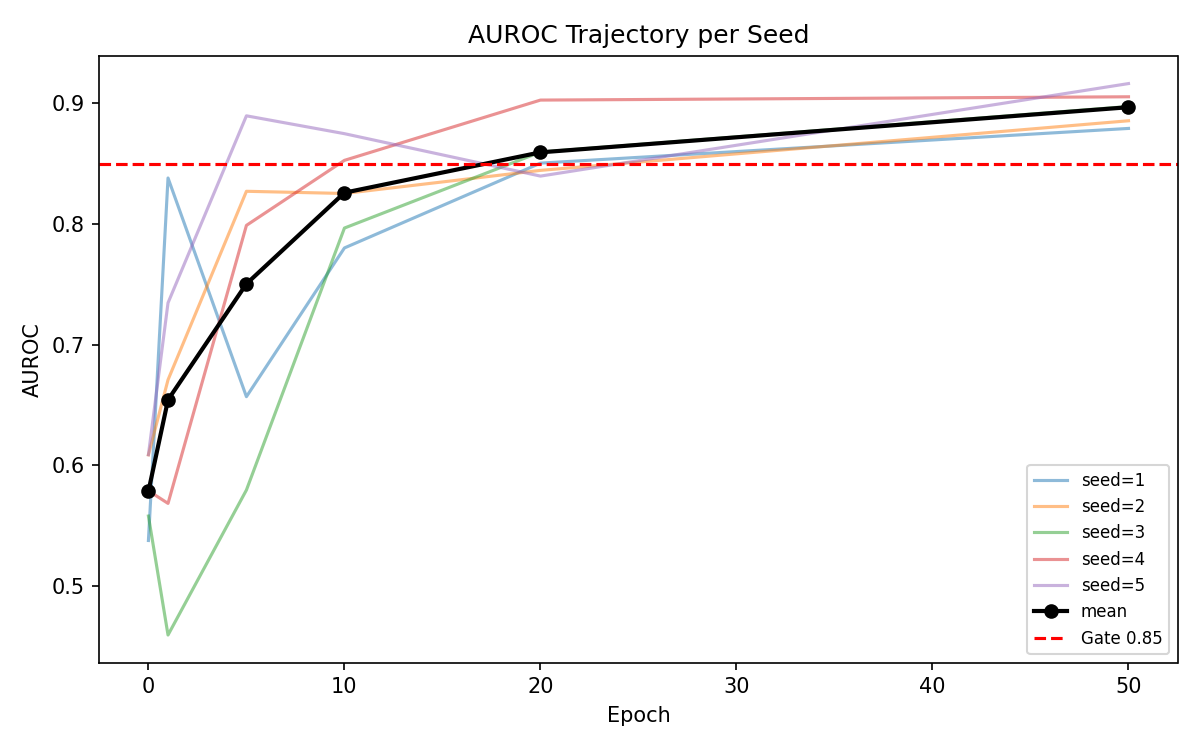
\includegraphics[width=\columnwidth]{figures/fig3_auroc_trajectory.png}
\caption{AUROC trajectory per seed}
\label{fig:fig3_auroc_trajectory}
\end{figure}

\textit{Figure 3: AUROC trajectory per seed across 6 checkpoints ($t\in {0,1,5,10,20,50})$. Dashed lines indicate gate thresholds at 0.70 (epoch-0 upper bound) and 0.85 (t} lower bound). Four of five seeds cross 0.85 by t\textit{.}

\#\#\#\# Estimator Stability

Hutchinson coefficient of variation (CV) across K=50 probes:

\begin{table}[htbp]
\centering
\resizebox{\columnwidth}{!}{%
\begin{tabular}{lll}
\toprule
Seed & CV & Stable? \\
\midrule
1 & 0.0233 & ✓ \\
2 & 0.0132 & ✓ \\
3 & 0.0232 & ✓ \\
4 & 0.0283 & ✓ \\
5 & 0.0108 & ✓ \\
\bottomrule
\end{tabular}
}
\end{table}

All CVs < 3\% (maximum 0.0283). K=50 Rademacher probes provide reliable per-sample trace estimates for the last-fc layer of ResNet-50. The trace signal is not dominated by Hutchinson estimation noise.

\begin{figure}[htbp]
\centering
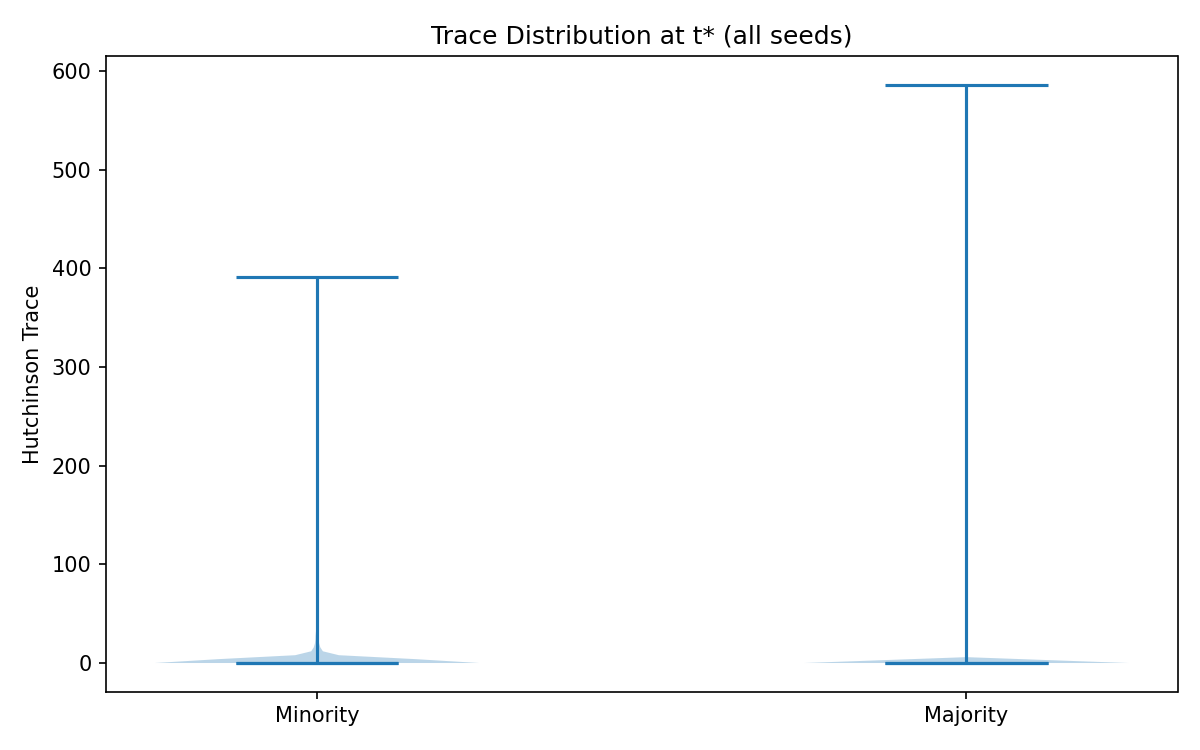
\includegraphics[width=\columnwidth]{figures/fig4_trace_distribution.png}
\caption{Per-sample trace distributions at t*}
\label{fig:fig4_trace_distribution}
\end{figure}

\textit{Figure 4: Per-sample Hessian trace distributions at t} for minority (groups 1+3) and majority (groups 0+2) training samples. Minority traces are systematically elevated, consistent with the empirical AUROC>0.85 finding.*

\begin{figure}[htbp]
\centering
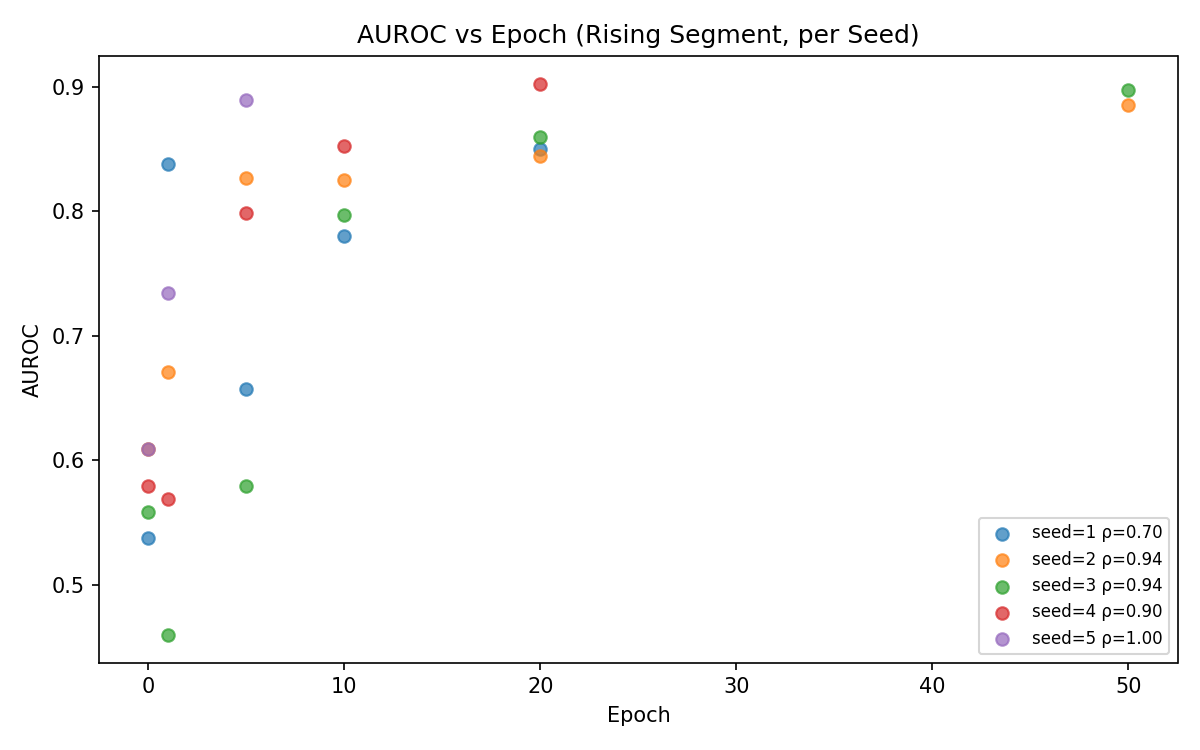
\includegraphics[width=\columnwidth]{figures/fig5_spearman_rising.png}
\caption{Spearman correlation per seed on rising segment}
\label{fig:fig5_spearman_rising}
\end{figure}

\textit{Figure 5: Spearman correlation on rising AUROC segment per seed. Seeds 2--5 achieve $\rho\geq 0.90$, confirming monotone rise. Seed 1 ($\rho$=0.70) shows a non-monotone trajectory at t=$1\rightarrow 5$.}

\subsubsection{5.2 H-M1: Confidence-Differential Mechanism Is Absent at t*}

\textbf{Main result:} The pre-registered mechanism gate fails in all 5 seeds. Minority training confidence at t* is 0.9678--0.9999 --- fully saturated, not boundary-straddling. The H-M1 gate is not satisfied.

\#\#\#\# Per-Seed Confidence at t*

\begin{table*}[htbp]
\centering
\resizebox{\dimexpr 2\columnwidth+\columnsep\relax}{!}{%
\begin{tabular}{llllll}
\toprule
Seed & t* & p\_minority(t*) & p\_majority(t*) & Confidence Gap & Boundary [0.3,0.7]? \\
\midrule
1 & 20 & 0.9956 & 0.9994 & 0.0039 & ✗ \\
2 & 50 & 0.9999 & 0.9999 & 0.0000 & ✗ \\
3 & 50 & 0.9998 & 0.9999 & 0.0000 & ✗ \\
4 & 20 & 0.9964 & 0.9992 & 0.0029 & ✗ \\
5 & 5 & 0.9678 & 0.9925 & 0.0247 & ✗ \\
\bottomrule
\end{tabular}
}
\end{table*}

\textbf{Gate result: FAIL (0/5 seeds).} No seed shows minority confidence in the predicted boundary condition range [0.3, 0.7] at t\textit{. Mean p\_minority(t})=0.9919, mean p\_majority(t*)=0.9982.

\#\#\#\# Full Confidence Trajectory (Seed 1)

\begin{table}[htbp]
\centering
\resizebox{\columnwidth}{!}{%
\begin{tabular}{llll}
\toprule
Epoch & p\_minority & p\_majority & Gap \\
\midrule
0 & 0.521 & 0.491 & 0.030 \\
1 & 0.827 & 0.972 & 0.145 \\
5 & 0.898 & 0.986 & 0.088 \\
10 & 0.964 & 0.996 & 0.032 \\
20 & 0.996 & 0.999 & 0.004 \\
50 & 1.000 & 1.000 & 0.000 \\
\bottomrule
\end{tabular}
}
\end{table}

\textbf{Transient early-epoch differential exists:} At epoch 1, a minority-majority confidence gap is visible (seed 1: p\_min=0.827 vs p\_maj=0.972, gap=0.145; seed 2: p\_min=0.720 vs p\_maj=0.975; seed 3: p\_min=0.570 vs p\_maj=0.967). This is consistent with LaBonte and Muthukumar [2026]'s Phase I prediction --- ERM learns the spurious feature first, temporarily lagging minority confidence. However, this differential disappears before t\textit{ in all seeds. By t}, both groups are saturated.

\begin{figure}[htbp]
\centering
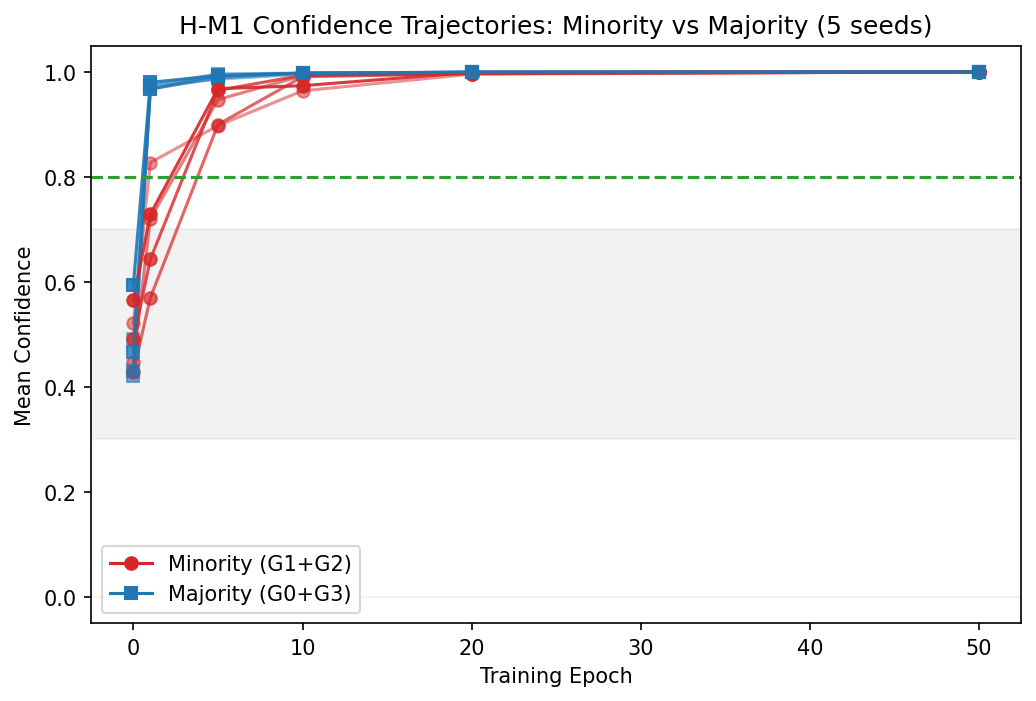
\includegraphics[width=\columnwidth]{figures/fig_confidence_trajectory.png}
\caption{Confidence trajectories per seed}
\label{fig:fig_confidence_trajectory}
\end{figure}

\textit{Figure 6: Training-set confidence trajectories for minority and majority groups per seed. At epoch 1, minority confidence lags majority (seed 1: p\_min=0.827 vs p\_maj=0.972). By t}, both groups saturate to $\geq 0.97$, refuting the sustained boundary-condition mechanism.*

\begin{figure}[htbp]
\centering
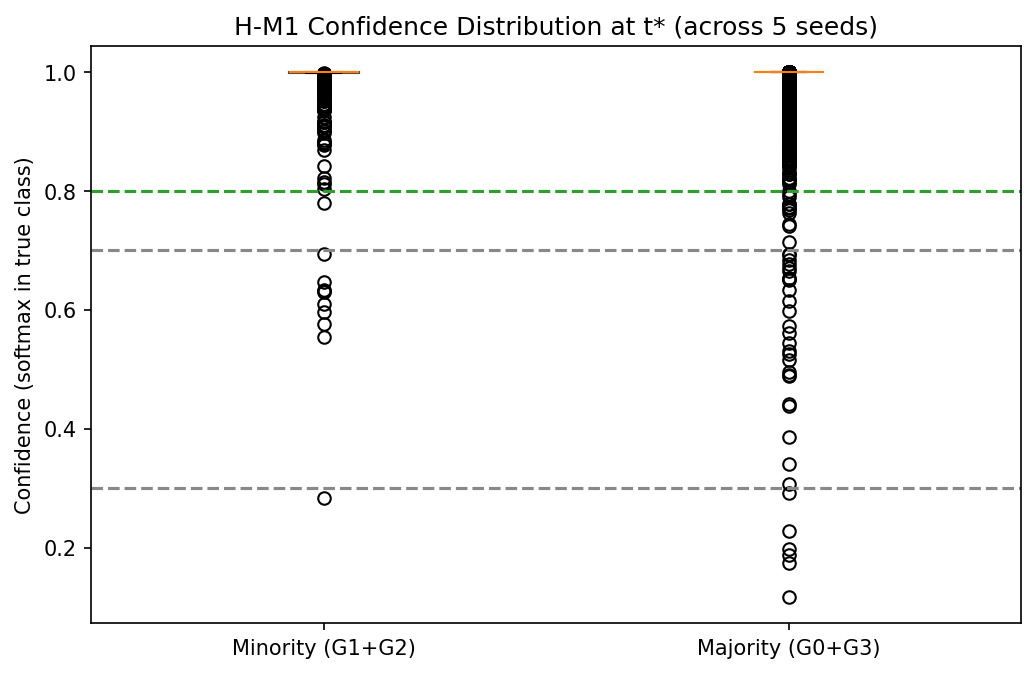
\includegraphics[width=\columnwidth]{figures/fig_conf_distribution.png}
\caption{Per-sample confidence distributions at t*}
\label{fig:fig_conf_distribution}
\end{figure}

\textit{Figure 7: Per-sample confidence distribution at t} for minority and majority samples. Both distributions are concentrated near 1.0 (mean p\_minority=0.9919, mean p\_majority=0.9982), demonstrating that the confidence channel p\_i($1-p_{i})$ is inactive at t\textit{.}

\begin{figure}[htbp]
\centering
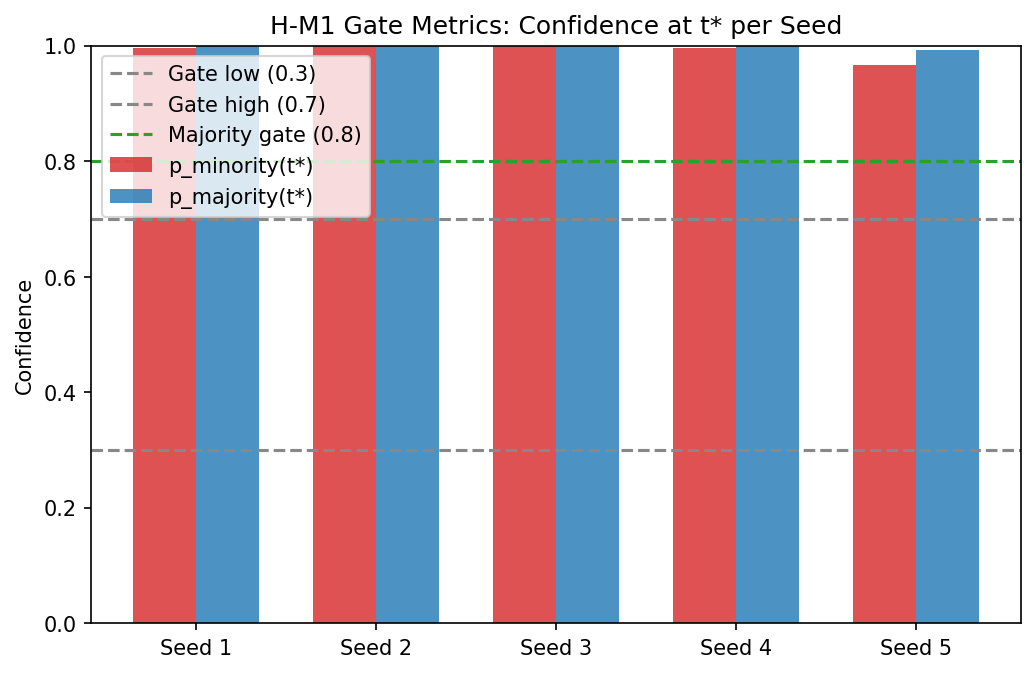
\includegraphics[width=\columnwidth]{figures/fig_gate_metrics.png}
\caption{H-M1 gate comparison}
\label{fig:fig_gate_metrics}
\end{figure}

\textit{Figure 8: H-M1 gate comparison: minority confidence at t} vs gate band [0.3, 0.7]. All 5 seeds show p\_minority(t\textit{)>0.96, with 0/5 seeds satisfying the boundary-condition criterion.}
